\chapter{Kalman-Filter}
\label{chap:KalmanFilter}

For the Kalman filter the noise of the measurement and the process has to be set up. This noise values are the variances of the used sensors and of the process. In the calculation process are those matrices named $\underline Q$ and $\underline R$. The matrix $\underline Q$ uses the variances of the process noise and the matrix $\underline R$ uses the variances of the noise of the sensors.\\\\
\underline{Prediction step:}\\\\
Predict the next state:
\begin{align}
\vec x_k = \underline{A}\vec x_{k-1}+\underline{B}\vec u_{k-1}
\label{equ:Kalman1}
\end{align}
Predict the covariance for the next step:
\begin{align}
\underline{P}_k = \underline{A}\underline{P}_{k-1}\underline{A}^T+\underline{Q}
\label{equ:Kalman2}
\end{align}
\underline{Correction step:}\\\\
Computation of the Kalman gain:
\begin{align}
\underline{K}_k = \underline{P}_k	\underline{H}^T(\underline{H}\underline{P}_k\underline{H}^T+\underline{R})^{-1}
\label{equ:Kalman3}
\end{align}
Updating state prediction with new measurement:
\begin{align}
\vec x_k = 	\vec x_k+\underline{K}_k(\vec z_k-\underline{H}\vec x_k)
\label{equ:Kalman4}
\end{align}
Updating the error covariance:
\begin{align}
\underline{P}_k = (\underline{I}-\underline{K}_k\underline{H})\underline{P}_k	
\label{equ:Kalman4}
\end{align}
As an initial guess the matrices are set to:
\begin{align}
\underline{Q} &= \begin{pmatrix} 0.005&0&0 \\ 0&0.005&0 \\ 0&0&0.0001 \end{pmatrix}\\
\underline{R} &= \begin{pmatrix} 0.5&0&0 \\ 0&0.5&0 \\ 0&0&0.01 \end{pmatrix}
\end{align}
With those matrices the following result was achieved. To make a test, first the yaw angle is changed in the range of $\pm90 \degree$, after that a roll angle is changed in the range of $\pm90 \degree$ and finally the pitch angle is changed in the range of $\pm90 \degree$. 

\begin{figure}[H]
	\centering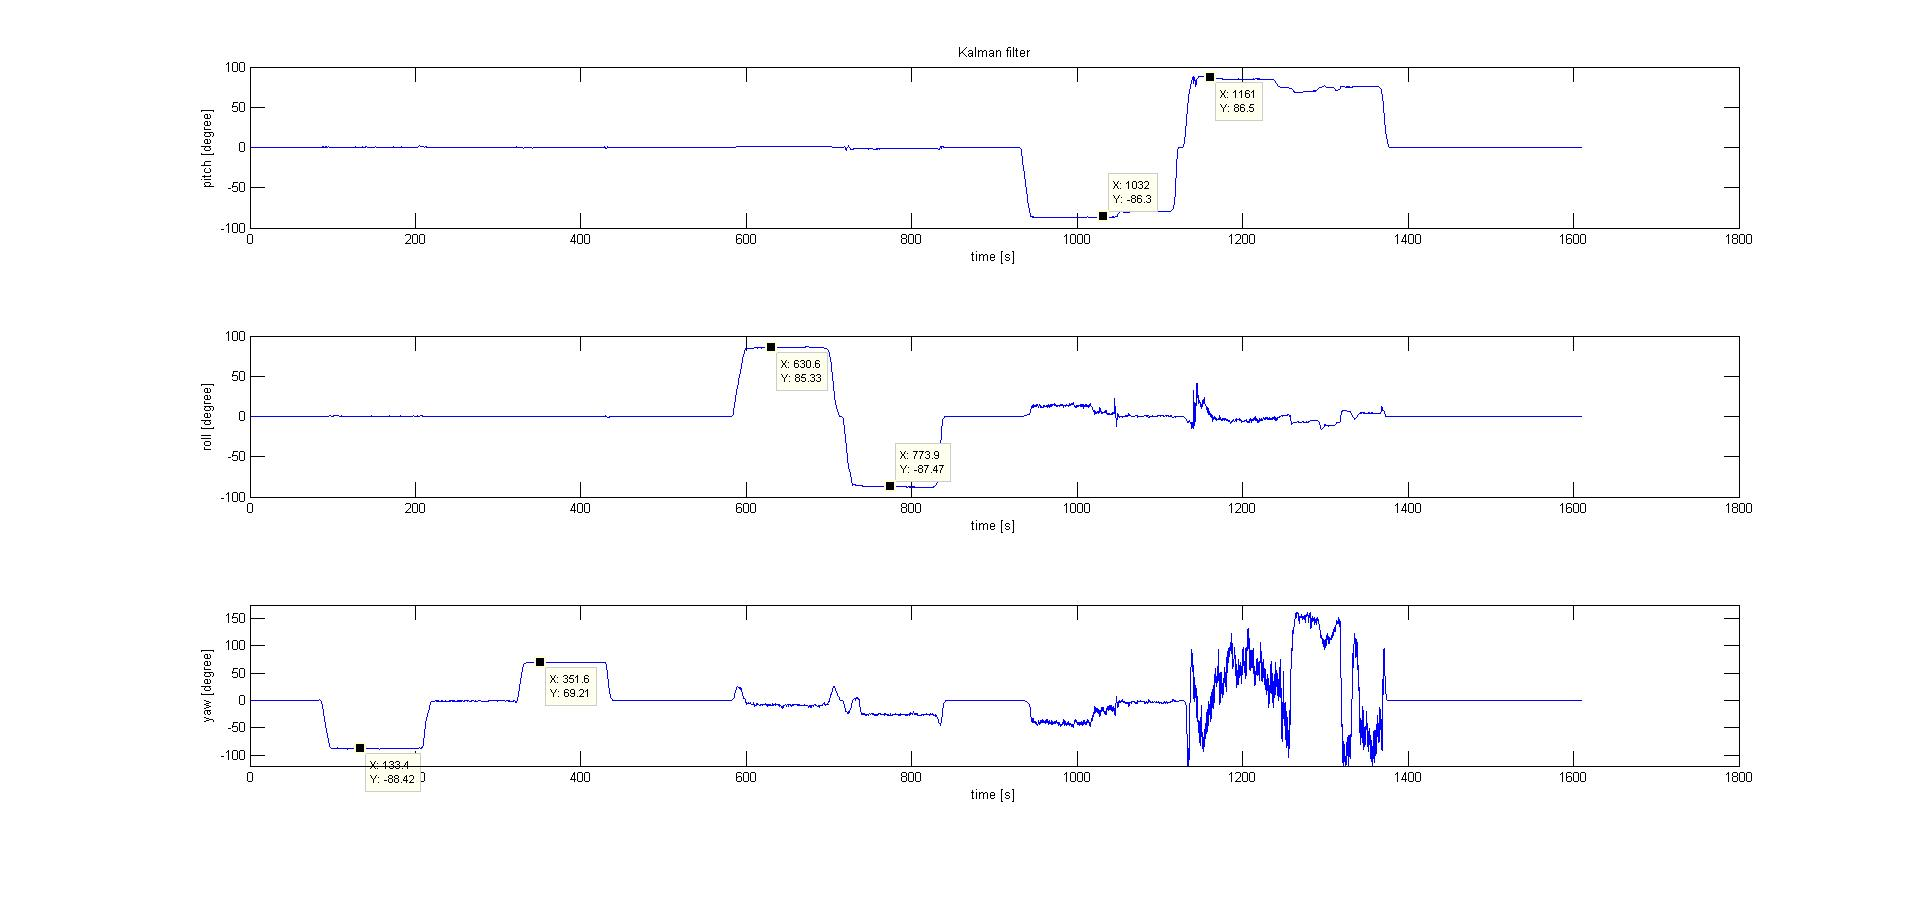
\includegraphics[width=1.0\textwidth]{fig/initial_Kalman}
	\caption{First result Kalman filter}
	\label{fig:initial_Kalman}
\end{figure}

The filter responses in a adequate time. Yaw angle change is like with the complementary filter from -90 degree to just 70 degree. The roll angle changes sufficient. But when changing the pitch angle to high a extreme yaw angle change can be seen. So the next step is to improve the yaw angle, so that it will reach also the +90 degree. Also the yaw change during pitch will be observed. After measuring the meanvalue and variances of all sensors they can be used to improve the Kalman filter. The figures \ref{fig:varAcc}, \ref{fig:varGyro} and \ref{fig:varMag} show the logged data.
\begin{figure}[H]
	\centering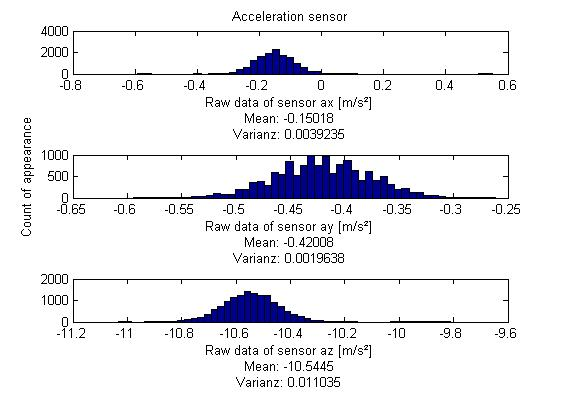
\includegraphics[width=0.8\textwidth]{fig/varAcc3}
	\caption{Analyzing the acceleration sensor}
	\label{fig:varAcc}
\end{figure}
\begin{figure}[H]
	\centering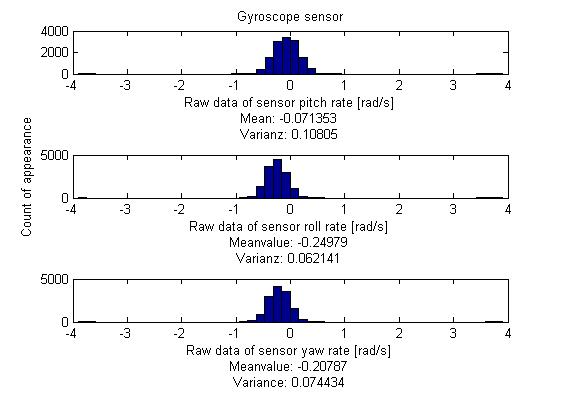
\includegraphics[width=0.8\textwidth]{fig/varGyro3}
	\caption{Analyzing the gyroscope sensor}
	\label{fig:varGyro}
\end{figure}
\begin{figure}[H]
	\centering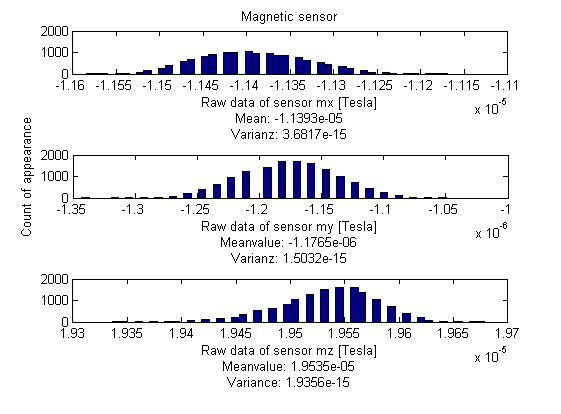
\includegraphics[width=0.8\textwidth]{fig/varMag3}
	\caption{Analyzing the magnetic sensor}
	\label{fig:varMag}
\end{figure}
First the matrix $\underline Q$, the variances of the process noise and the matrix $\underline R$, the variances of the measured sensor noises are changed by using the measured values. The new values are:\\
\begin{align}
\underline{Q} &= \begin{pmatrix} 0.005&0&0 \\ 0&0.005&0 \\ 0&0&0.005 \end{pmatrix}\\
\underline{R} &= \begin{pmatrix} 0.06&0&0 \\ 0&0.1&0 \\ 0&0&0.07 \end{pmatrix}
\end{align}

\begin{figure}[H]
	\centering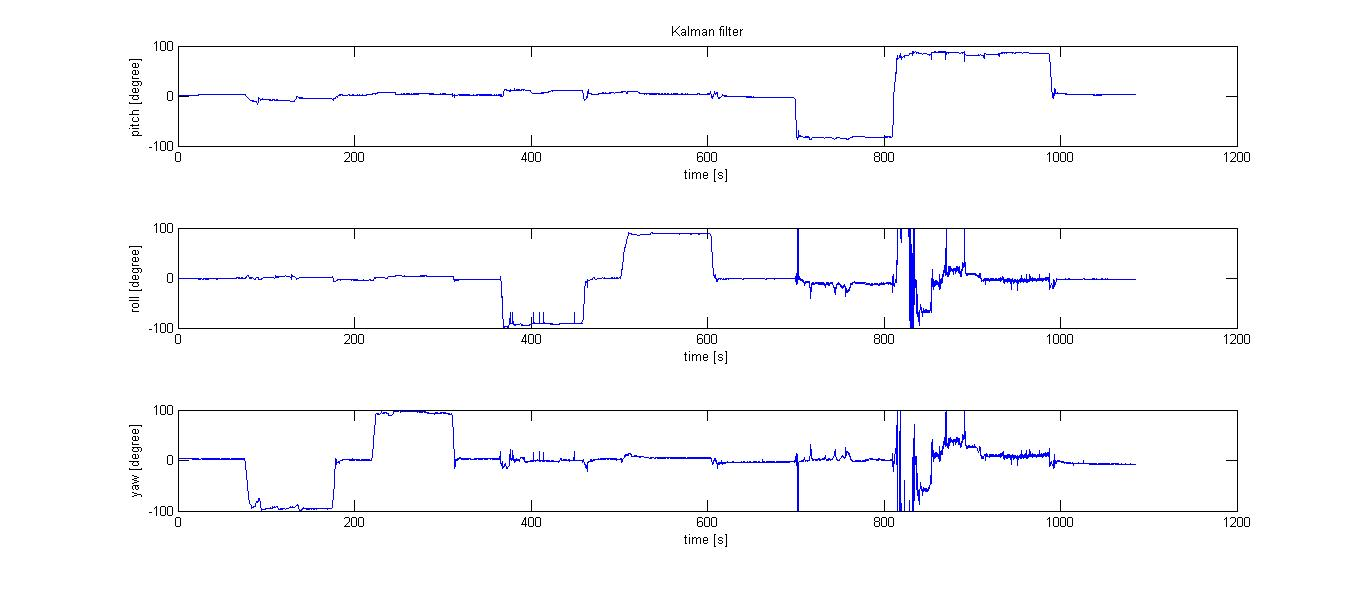
\includegraphics[width=1.0\textwidth]{fig/final_Kalman1}
	\caption{Final result Kalman filter}
	\label{fig:final_Kalman}
\end{figure}
The wanted improving of the yaw angle in reaching the 90 degree when turning 90 degree is succesfully reached. The extreme influences on yaw directly after changing of the rotation angle results from a hand made rotation. The influences on yaw while an other angle is applied is extremely reduced.\\

The last figure shows how off an angle can be when just an gyroscope is used. On the left side the integrated gyroscope can be seen. On the right side, the 3D representation of the fusioned sensors are displayed.
\begin{figure}[H]
	\centering\includegraphics[width=0.6\textwidth]{fig/3D}
	\caption{3D representation of the integrated gyroscope raw values on the left and the fusion filtered on the right}
	\label{fig:3D}
\end{figure}